\nsection{Problem 2 - (EM-algorithm)}
We will now assume that the data $Y_i, i=1, \ldots n$, are independent and identically distributed according to the mixture distribution:
$$
f\left(y_i\right)=p \cdot \phi\left(y_i ; 0,1^2\right)+(1-p) \cdot \phi\left(y_i ; 0, \tau^2+1^2\right)
$$
where $\phi\left(y_i ; \mu, \sigma^2\right)$ is the normal density with mean $\mu$ and variance $\sigma^2$. We will now consider estimation of the parameters $\theta=\left(p, \tau^2\right)$.
\nssection{a.)}
\emph{Give an expression for the likelihood of $\theta$.} \spaze
\textbf{Solution:} \spaze
We recall that the likelihood function of a parameter $\theta$ is given by 
\begin{align}
    L(\theta| y_i) =\prod_{i=1}^{n} f(y_i) 
\end{align}
where $f(y_i)$ refers to the probability mass function of $y_i$. Hence by direct insertion we have that 
\begin{align*}
     L(\theta| y_i) &=\prod_{i=1}^{n} f(y_i)  \\[5pt]
     &= \prod_{i=1}^{n} \left[ p \cdot \phi\left(y_i ; 0,1^2\right)+(1-p) \cdot \phi\left(y_i ; 0, \tau^2+1^2\right) \right]
\end{align*}
and we are done. $\Q$
\nssection{b.)}
\emph{Introduce the variable $C_i$ which identify which of the two modes $y_i$ belongs to. Give an expression for the complete log-likelihood using the pairs $\left(C_i, y_i\right), \ i=1, \ldots n$} \spaze
\textbf{Solution:} \spaze
Given the Likelihood function of our mixture distribution (i.e 2a):
\[
L(\theta| y_i) = \prod_{i=1}^{n} \left[ p \cdot \phi\left(y_i ; 0,1^2\right)+(1-p) \cdot \phi\left(y_i ; 0, \tau^2+1^2\right) \right]
\]
We aim to derive the complete log-likelihood function when introducing the variable \( C_i \), which identifies which of the two modes \( y_i \) belongs to. The indicator variable \(C_i\) is a binary variable, defined accordingly
\[
C_i = 
\begin{cases}
0, & \text{if } y_i \text{ belongs to the first mode,} \\
1, & \text{if } y_i \text{ belongs to the second mode.}
\end{cases}
\]
Furthermore, is it understood that $C_i$ takes on the given values with probabilities
\begin{align*}
    \mathbb{P}(C_i) = p \iff C_i = 1 \iff y_i \ \text{belongs to the second mode} \\[5pt]
    \mathbb{P}(C_i) = 1-p \iff C_i = 0 \iff y_i \ \text{belongs to the first mode}
\end{align*}
From here we start of by converting the Likelihood function to a log-likelihood 
\begin{align}
    \ell(\theta|y) &= \log\left(L(\theta|y) \right) \\[5pt]
    &= \log \left(\prod_{i=1}^{n} \left[ p \cdot \phi\left(y_i ; 0,1^2\right)+(1-p) \cdot \phi\left(y_i ; 0, \tau^2+1^2\right) \right] \right) \\[5pt]
    &= \sum_{i=1}^{n} \log \left[ p \cdot \phi\left(y_i ; 0,1^2\right)+(1-p) \cdot \phi\left(y_i ; 0, \tau^2+1^2\right) \right]
\end{align}
Observing that for each \(y_i\), only one term is chosen from the probability density function, based on the mode for that \(y_i\). Meaning thus that we interpret \(C_i\) as an indicator function. By logarithmically transforming both terms, we obtain the complete log-likelihood function for the observed and missing data pairs \((C_i, Y_i)\), \(i = 1, \ldots, n\), expressed as: 
\begin{align*}
\ell(\theta | y_i, C_i) &= \sum_{i=1}^{n} \left[ C_i \cdot \log\left(p \cdot \phi\left(y_i ; 0,1^2\right)\right) + (1 - C_i) \cdot \log\left((1-p) \cdot \phi\left(y_i ; 0, \tau^2+1^2\right)\right) \right]
\end{align*}
And we are done. $\Q$
\nssection{c.)}
\emph{Give an expression for $Q\left(\theta \mid \theta^{(t)}\right)$, what is the interpretation of $Q\left(\theta \mid \theta^{(t)}\right)$. Derive the estimates for $\theta=\left(p, \tau^2\right)$, using $Q\left(\theta \mid \theta^{(t)}\right)$.} \spaze
\textbf{Solution:} \spaze
To rigidly express $Q\left(\theta | \theta^{(t)}\right)$, we start off by looking at the conditional probabilities of $C_i$ given the observation on $y_i$. \vspace{3mm}\\ 
The probability that $C_i = 0$ given the observation on $y_i$ is: 
\begin{align}
    \mathbb{P}(C_i = 0 | y_i, \theta^{t}) = \frac{(1-p)\cdot \phi\left(y_i ; 0, \tau^2+1^2\right)}{p \cdot \phi\left(y_i ; 0,1^2\right)+(1-p) \cdot \phi\left(y_i ; 0, \tau^2+1^2\right)} 
\end{align}
Analogously is the probability that $C_i = 1$ given the observation on $y_i$ expressed as:
\begin{align}
    \mathbb{P}(C_i = 1 | y_i, \theta^{t}) = \frac{p \cdot \phi\left(y_i ; 0,1^2\right)}{p \cdot \phi\left(y_i ; 0,1^2\right)+(1-p) \cdot \phi\left(y_i ; 0, \tau^2+1^2\right)}
\end{align}
Henceforth we proceed to compute the expected value of the joint log-likelihood function of the complete dataset, denoted by $Q\left(\theta | \theta^{(t)}\right)$ 
\begin{align}
    Q\left(\theta | \theta^{(t)}\right) &= \mathbb{E}\bl \log L(\theta | y) \mid y, \theta^{(t)}\br \\[5pt]
    &= \begin{aligned}[t]
       & \sum_{i=1}^{n} \mathbb{P}(C_i = 1 | y_i, \theta^{(t)}) \log\left(p \cdot \phi\left(y_i ; 0,1^2\right)\right) \\
       & + \mathbb{P}(C_i = 0 | y_i, \theta^{(t)}) \log\left((1-p) \cdot \phi\left(y_i ; 0, \tau^2+1^2\right)\right)
       \end{aligned}
\end{align}
The Q-function computes the expected complete log-likelihood using both the observed data and the current parameter estimates. By maximizing the Q-function, we adjust the parameters to maximize the expected complete log-likelihood. \spaze
To derive the estimates for $\theta$ we need to maximize $Q(\theta|\theta^{(t)})$ with respect to $\theta$ itself. By ease of notation we define the maximizer to be $\theta^{(t+1)} = \left(p^{(t+1)}, \tau^{{2}^{(t+1)}} \right)$. \spaze 
Initially, we look at the derivative of $Q$ with respect to $p$: 
\begin{align}
    \frac{\partial }{\partial p} Q(\theta| \theta^{(t)}) &= \frac{\partial }{\partial p} \left[ \begin{aligned}[t]
       & \sum_{i=1}^{n} \mathbb{P}(C_i = 1 | y_i, \theta^{(t)}) \log\left(p \cdot \phi\left(y_i ; 0,1^2\right)\right) \\
       & + \mathbb{P}(C_i = 0 | y_i, \theta^{(t)}) \log\left((1-p) \cdot \phi\left(y_i ; 0, \tau^2+1^2\right)\right)
       \end{aligned} \right] \\[10pt]
       &= \sum_{i=1}^{n} \left[ \frac{{\mathbb{P}(C_i = 1 | y_i, \theta^{(t)})}}{{p}} - \frac{{\mathbb{P}(C_i = 0 | y_i, \theta^{(t)})}}{{1-p}} \right]
\end{align} 
then multiply by $p(1-p)$ 
\begin{align*}
    \sum_{i=1}^{n} (1-p) \mathbb{P}\left(C_i = 1 | y_i, \theta^{(t)}\right) - p \left( \mathbb{P}\left(C_i = 0 | y_i, \theta^{(t)}\right) \right)
\end{align*}
which by expansion of the first term yields 
\begin{align*}
     \sum_{i=1}^{n} \mathbb{P}\left(C_i = 1 | y_i, \theta^{(t)}\right) - p \left( \mathbb{P}\left(C_i = 1 | y_i, \theta^{(t)}\right) \right) - p \left( \mathbb{P}\left(C_i = 0 | y_i, \theta^{(t)}\right) \right)
\end{align*}
and through factoring for $p$ 
\begin{align*}
    \sum_{i=1}^{n} \mathbb{P}\left(C_i = 1 | y_i, \theta^{(t)}\right) - p \left( \mathbb{P}\left(C_i = 1 | y_i, \theta^{(t)}\right) + \mathbb{P}\left(C_i = 0 | y_i, \theta^{(t)}\right)\right)
\end{align*}
whereby setting the expression equal to zero conclusively gives 
\begin{align*}
    & \sum_{i=1}^{n} \mathbb{P}\left(C_i = 1 | y_i, \theta^{(t)}\right) - p \left( \mathbb{P}\left(C_i = 1 | y_i, \theta^{(t)}\right) + \mathbb{P}\left(C_i = 0 | y_i, \theta^{(t)}\right)\right) = 0 \\[8pt]
    & \hspace{5cm} \Updownarrow \\[8pt]
    & p \left( \sum_{i=1}^{n}  \mathbb{P}\left(C_i = 1 | y_i, \theta^{(t)}\right) + \mathbb{P}\left(C_i = 0 | y_i, \theta^{(t)}\right) \right) = \sum_{i=1}^{n} \mathbb{P}\left(C_i = 1 | y_i, \theta^{(t)}\right)
\end{align*}
meaning 
\begin{align*}
    p = \frac{\sum_{i=1}^{n} \mathbb{P}\left(C_i = 1 | y_i, \theta^{(t)}\right)}{\sum_{i=1}^{n}  \mathbb{P}\left(C_i = 1 | y_i, \theta^{(t)}\right) + \mathbb{P}\left(C_i = 0 | y_i, \theta^{(t)}\right)}
\end{align*}
which says that the updating rule on $p$ is 
\begin{align}
    p^{(t+1)} = \frac{1}{n} \sum_{1}^{n} \frac{p^{(t)} \cdot \phi\left(y_i ; 0,1^2\right)}{p^{(t)} \cdot \phi\left(y_i ; 0,1^2\right)+(1-p^{(t)}) \cdot \phi\left(y_i ; 0, \tau^2+1^2\right)}.
\end{align}
Similarly, we proceed by differentiating $Q$ with respect to $\tau^2$:
\begin{align}
    \frac{\partial }{\partial \tau^2} Q (\theta | \theta^{(t)}) = \sum_{i=1}^{n} (1 - p) \left(\frac{y_{i}^2}{(\tau^2 +1)^2} - \frac{1}{\tau^2 + 1} \right)
\end{align}
\footnote{This result comes from the fact that the Gaussian density function \(\phi(\cdot ; \mu, \sigma^2)\) has the derivative:
\[\frac{d}{d\sigma^2} \phi(x ; \mu, \sigma^2) = \frac{(x - \mu)^2}{\sigma^4} \phi(x ; \mu, \sigma^2) - \frac{1}{\sigma^2} \phi(x ; \mu, \sigma^2)\]} and equating to zero
\begin{align*}
    &\sum_{i=1}^{n} (1 - p) \left(\frac{y_{i}^2}{(\tau^2 +1)^2} - \frac{1}{\tau^2 + 1} \right) = 0 \\[5pt]
    &\sum_{i=1}^{n}  (1 - p) \left( \frac{y_{i}^2 - (\tau^2 + 1)}{(\tau^2 +1)^2}\right) =  0 \\[5pt]
     & \hspace{2cm} \Downarrow \\[5pt]
     &\sum_{i=1}^{n}  (1 - p) \left( y_{i}^2 - (\tau^2 + 1)\right) = 0 \\[5pt]
      & \hspace{2cm} \Updownarrow \\[5pt]
      &\sum_{i=1}^{n}  (1 - p) y_{i}^2 =  \sum_{i=1}^{n}  (1 - p) (\tau^2 + 1) \\[5pt]
      & \hspace{2cm} \Downarrow \\[5pt]
        &\tau^2 + 1 =  \frac{\sum_{i=1}^{n} (1 - p) y_{i}^2}{\sum_{i=1}^{n}1-p} 
\end{align*}
thus yielding 
\begin{align*}
    \tau^2 = \frac{\sum_{i=1}^{n} (1 - p) y_{i}^2}{\sum_{i=1}^{n}1-p}  - 1
\end{align*} 
Meaning the updating rule on $\tau^2$ is then 
\begin{align}
\tau^{{2}^{(t+1)}} = \frac{\sum_{i=1}^{n} (1 - p) y_{i}^2}{\sum_{i=1}^{n} 1-p}  - 1
\end{align}
and we are done. $\Q$
\nssection{d.)}
\emph{ Implement the solution you derived in c) as a function and apply it to the data:} \texttt{sparseDataWithErrors.dat}

\emph{What is a good initialization?} \spaze

\textbf{Solution:} \spaze
A natural assumption on initialization is to assume that the modes are equal and that the data points are evenly distributed between them. Hence set $p = 0.5$ and $\tau^2 = 0$. More generally we could assume an initialization of $p \in (0,1)$ (due to it being a probability), and $\tau^2 \neq 1$ (to avoid identical distribution). \\

The implementation can be found in Appendix \ref{appendix:b}, from code listing  (\ref{lst:EM-alg}). The code produces the following result:
\begin{align*}
    (p, \tau^2) = (0.946004, 75.005977)
\end{align*}
where a section of the iteration show the following progression 
\begin{table}[H]
\centering
\begin{tabular}{SSS} \toprule
{$i$} & {$p$} & {$\tau^2$} \\ \midrule
1 & 0.5 & 3 \\ \hline
5 & 0.862589 & 30.258267 \\ \hline
10 & 0.944501 & 73.045733\\ \hline
15 & 0.945983 & 74.977963 \\ \hline
20 & 0.946004 & 75.005588\\ \hline
30 & 0.946004 & 75.005977 \\ \hline
\end{tabular}
\caption{Iterative estimation of $p$ and $\tau^2$ where $i$ denotes the number of iterations}
\label{tab:iterative_approx}
\end{table}
As presented above we see that even for quite low values of $p$ and $\tau^2$, the algorithm converges quickly within around 30 iterations, which of course can be reduced even more given that the starting values are closer to the realised ones. 
\nssection{e.)}
\emph{Compute a bootstrap estimate of the uncertainty of the two parameters, using the function from d. Sample $B=1000$ times and display scatter plot of the values.} \spaze
\textbf{Solution:} \spaze
The implementation can be found in Appendix \ref{appendix:b}, from code listing  (\ref{lst:tau_p_est}). The code produces the following plot: 
\begin{figure}[H]
  \centering
  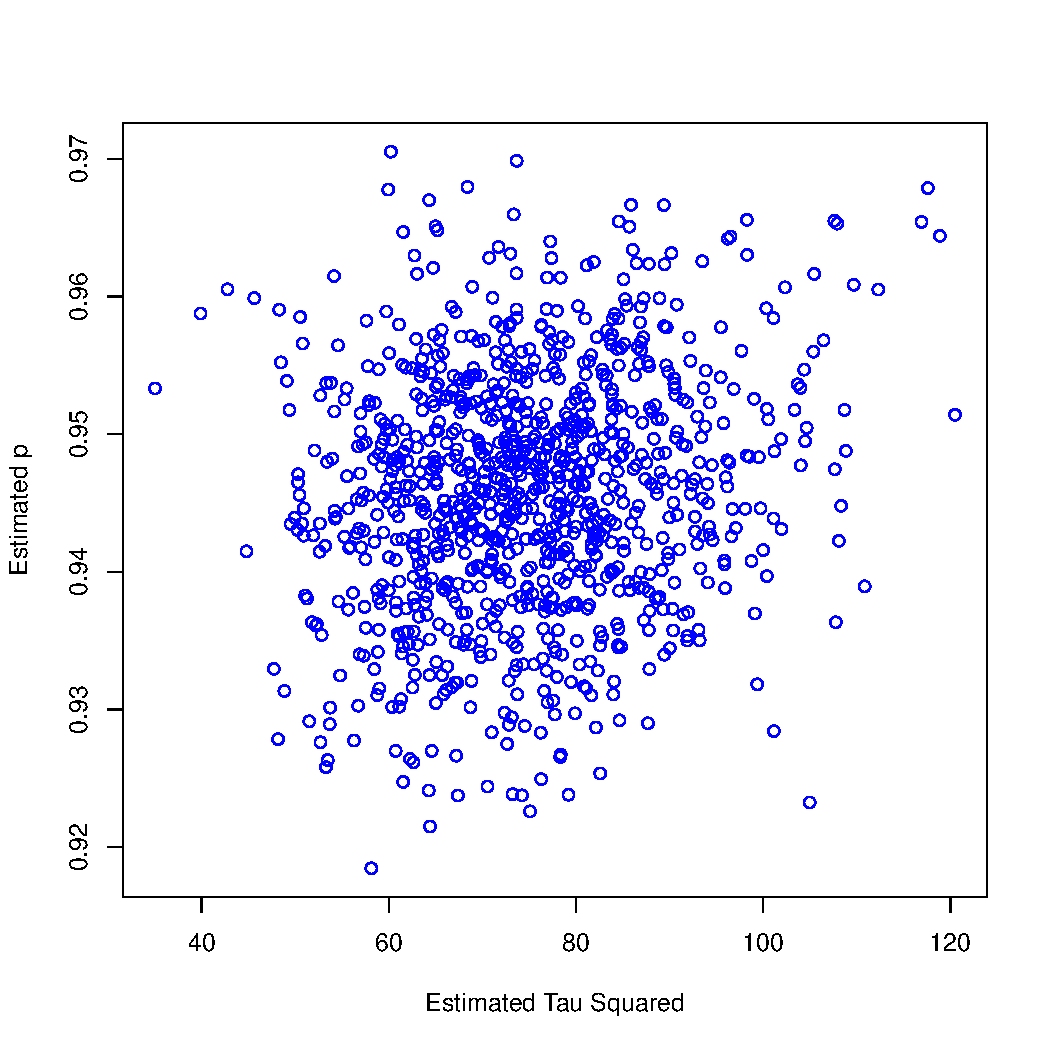
\includegraphics[width=0.6\textwidth]{Images/Figures_Exercise_2/bootstrap_results-seed.pdf}
  \caption{Scatter plot of bootstrap estimations for $\tau^2$ and $p$}
  \label{fig:boot_scat}
\end{figure}
whereby constructing 95 $\%$ confidence intervals for $p$ and $\tau^2$ yield 
\begin{align}
    \mathbb{P}_{p} \left(0.9278386  \leq p \leq  0.9631131\right) &= 95 \% \\[5pt]
      \mathbb{P}_{\tau^2} \left(  51.4844 \leq \tau^2 \leq  103.3594 \right) &= 95 \% 
\end{align}
It is observed that there is notably higher uncertainty associated with $\hat{\tau}^2$ compared to $\hat{p}$, which is understandable given that the predicaments of the 95 $\%$ confidence interval for $p$ admit values of $p > 0.925$, implying that fewer than 75 samples belong to mode 2. Moreover, the width of $\mathbb{P}_{\tau^2}$ naturally tells us that there are clear indications of instability in the estimate of $\tau^2$.
\nssection{f.)}
\emph{Compute the observed information matrix. How can you use the observed information matrix to give an uncertainty estimate for $\theta$? Compare the result to e.} \spaze
\textbf{Solution:} \spaze
To approach this computation it is necessary to define exactly what we want to compute, correctly. We are working with a "true" parameter $\theta$, a consistent estimate $\hat{\theta}$ (from 2c and 2d), the expected (fisher) information $I(\theta)$ at $\theta$ and the observed (fisher) information $\mathcal{J}(\theta)$ at $\theta$. \spaze
What then needs to be established is that all of these quantities are asymptotically equivalent, respectively. This means that given enough samples (data), the observed fisher information will in probability converge to the expected fisher information and likewise the consistent estimate to the true parameter. More mathematically this says that 
\begin{align}
    \mathcal{J}(\theta) &= \frac{1}{n} \sum_{i=1}^{n} \frac{\partial^2}{\partial \theta^2} \ell(\theta|y) \qquad \text{(Observed Fisher information)} \\[5pt]
    \lim_{n \to \infty}  \mathcal{J}(\theta) &= \lim_{n \to \infty} \frac{1}{n} \sum_{i=1}^{n} \frac{\partial^2}{\partial \theta^2} \ell(\theta|y) \\[5pt] 
    &= \mathbb{E}_{\theta} \left( \frac{\partial^2}{\partial \theta^2} \ell(\theta|y) \right) \qquad \text{(Expected Fisher information)}.
    \end{align}
The assured convergence follows directly from the law of large numbers. \spaze 
Since we are primarily looking at using the full dataset in this exercise, there will therefore not be a distinct difference between the two measures and can hence express the observation matrix accordingly 
\begin{align*}
    \mathcal{J}(\theta) &= -\nabla \nabla \ell(\theta) \\[5pt]
    &= - H_{\ell}
\end{align*}
where $H_{\ell}$ is the Hessian matrix of the log-likelihood with respect to the parameter $\theta$. In our case the Hessian is simply a $2 \times 2$ matrix, with elements 
\begin{align}
    H_{\ell} = \begin{pmatrix}
                        \frac{\partial^2 \ell(\theta)}{\partial p^2} &  \frac{\partial^2 \ell(\theta)}{\partial p \partial \tau^2} \\[7pt]
                         \frac{\partial^2 \ell(\theta)}{\partial \tau^2 \partial p} & \frac{\partial^2 \ell(\theta)}{\partial (\tau^2)^2}
                \end{pmatrix}.
\end{align}
By construction of $\ell(\theta|y)$ it is too tedious to compute $H_{\ell}$ analytically, and we will numerically approximate it instead. The implementation can be found in Appendix \ref{appendix:b}, from code lisitings (\ref{lst:fisher_inf}). Where the resulting observation matrix becomes 
\begin{align*}
     \mathcal{J}(\theta) &= \begin{pmatrix}
          13693.156468 & -1.896655 \\[5pt]
          -1.896655  & 0.004318338
     \end{pmatrix}
\end{align*}
The Negative values admitted in \( \mathcal{J}(\theta) \) \footnote{I am not completely certain that this is correct, so if not I would fully appreciate a more thorough explanation and result} for \( \frac{\partial^2 \ell(\theta)}{\partial \tau^2 \partial p} \) indicate potential anomalies in the data, where \( p \) and \( \tau^2 \) might show significant correlation. This implies that specific care in interpretation of the diagonal elements, which represent mean square error (due to proportionality), is recommended. \spaze
The related covariance matrix, or the inverse of the observation matrix, further establishes the aforementioned: 
\begin{align*}
    \mathcal{J}^{-1}(\theta) = \text{Cov}(\theta) = \begin{pmatrix}
          7.775973 \cdot 10^{-5} & 0.03415281 \\[5pt]
          0.03415281  & 246.57082498
     \end{pmatrix}
\end{align*}
\nssection{g.)}
\emph{Compute the likelihood from $2 \mathrm{a}$, in a dense grid $\left(p, \tau^2\right) \in[0.8,1] \times[50,130]$. Normalize it by dividing by the maximum value and plot it in a contour plot. Use contours lines [0.01 0.1 0.5 0.95], mark the ML estimator in the plot. Compare the results to e and f.} \spaze
\textbf{Solution:} \spaze
The implementation can be found in Appendix \ref{appendix:b}, from code lisitings (\ref{lst:contour_plot}). It produces the following plot
\begin{figure}[H]
  \centering
  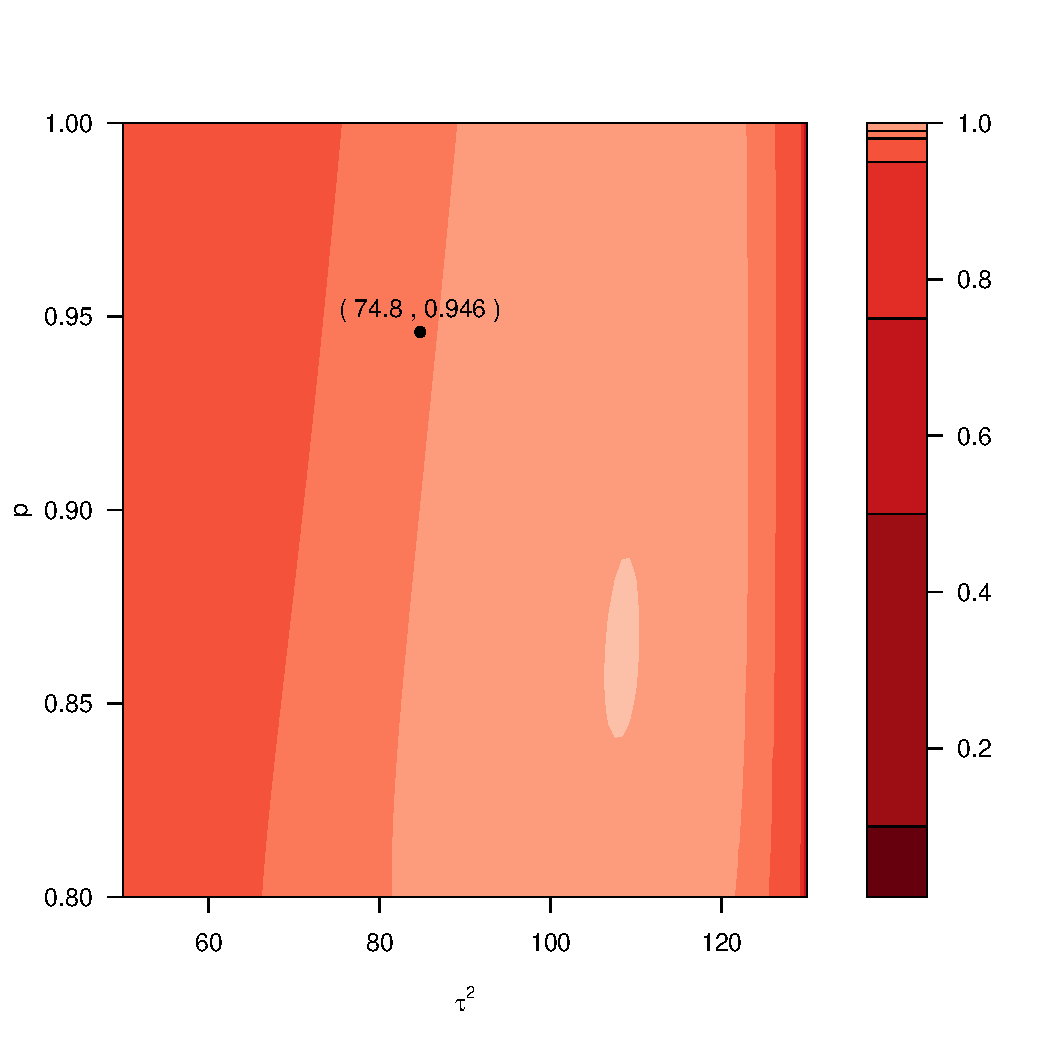
\includegraphics[width=0.7\textwidth]{Images/Figures_Exercise_2/contour_plot.pdf}
  \caption{Contour plot of of $L(\theta|y)$ in the grid $\left(p, \tau^2\right) \in[0.8,1] \times[50,130]$}
  \label{fig:contour_plot}
\end{figure}
which compares well to the estimates from our bootstrap for the MLE. 